\documentclass[11pt,a4paper]{ctexart}

\usepackage[a4paper,margin=1in]{geometry}
\usepackage{fontspec}
\usepackage{booktabs}
\usepackage{array}
\usepackage{longtable}
\usepackage{hyperref}
\usepackage{enumitem}
\usepackage{xcolor}
\usepackage{graphicx}
\usepackage{float}
\usepackage{listings}

\setmainfont{DejaVu Serif}
\setCJKmainfont{Droid Sans Fallback}
\setmonofont{DejaVu Sans Mono}

\lstset{
    basicstyle=\ttfamily\small,
    commentstyle=\ttfamily\small,
    breaklines=true,
    frame=single,
    columns=fullflexible,
    keepspaces=true,
    showstringspaces=false
}

\hypersetup{
    colorlinks=true,
    linkcolor=blue,
    urlcolor=blue
}

\title{CS305 SDN Project Report（中文版）}
\author{
    Tong Wu (12412460) \and
    Zhikai Wang (12410615) \and
    Yunzang Li (12410922)
}
\date{\today}

\begin{document}

\maketitle

\section{项目简介}

本项目基于 os-ken 与 Mininet 实现了一个集中式 SDN 控制器。网络被建模为单子网的二层环境，包含主机与 OpenFlow 交换机。控制器支持三项必做功能：

\begin{itemize}[leftmargin=1.5em]
    \item 基于 DHCP 的动态地址分配；
    \item 基于当前拓扑的最短路径转发；
    \item 基于交换机流表的防火墙过滤。
\end{itemize}

在必做部分之外，我们还实现了多个 bonus，包括 DNS 支持、DHCP 租约增强、TCP 拥塞控制实验以及 bufferbloat 实验。

\section{系统架构}

整个系统以集中式控制器为核心。Mininet 负责创建虚拟主机、交换机与链路；os-ken 控制器维护全局拓扑视图，并将 OpenFlow 规则下发到交换机中。主机负责产生业务流量，而控制器负责决定网络应当如何响应。

从功能上看，系统可以分为四层：

\begin{itemize}[leftmargin=1.5em]
    \item \textbf{拓扑与转发层}：维护交换机、链路和主机状态；计算最短路径；安装转发表。
    \item \textbf{DHCP 层}：处理 DHCP 报文，管理地址分配、pending offer、正式租约与续租。
    \item \textbf{防火墙层}：从 JSON 规则文件中解析 deny 规则，并下发高优先级丢弃流表。
    \item \textbf{Bonus DNS 层}：按照静态 DNS 记录表响应域名查询。
\end{itemize}

\subsection{核心文件}

\begin{itemize}[leftmargin=1.5em]
    \item \texttt{controller.py}：控制器主逻辑，处理交换机、主机、链路、端口与数据包事件，并协调 DHCP、DNS、ARP、最短路和防火墙规则安装。
    \item \texttt{dhcp.py}：DHCP 服务器实现，包含地址分配、租约管理、超时回收与续租逻辑。
    \item \texttt{firewall.py}：防火墙规则解析与流表安装逻辑。
    \item \texttt{dns\_server.py}：控制器侧 bonus DNS 实现。
    \item \texttt{ofctl\_utilis.py}：OpenFlow 辅助工具，负责流表安装和 PacketOut 发送。
    \item \texttt{tests/}：Mininet 测试脚本，覆盖必做和 bonus 部分。
\end{itemize}

\subsection{控制逻辑}

控制器维护以下共享状态：

\begin{itemize}[leftmargin=1.5em]
    \item 在线 datapath 与 OpenFlow 控制抽象；
    \item 学习到的主机位置以及 IP 到 MAC 的映射；
    \item 交换机邻接关系；
    \item 交换机间端口映射；
    \item 用于拓扑刷新和故障处理的 down-port 集合。
\end{itemize}

在此基础上，控制器根据主机位置与交换机拓扑计算最短路径，并按照目的 MAC 下发转发规则。

\section{实现细节}

\subsection{DHCP}

DHCP 模块实现了标准的 DISCOVER/OFFER/REQUEST/ACK 流程。测试脚本中的主机初始并不带有效 IP，因此地址分配必须由控制器侧完成。

\texttt{dhcp.py} 中维护了如下状态：

\begin{itemize}[leftmargin=1.5em]
    \item pending offers；
    \item 已确认租约；
    \item 租约过期时间戳；
    \item 被客户端拒绝、不得再次分配的地址。
\end{itemize}

在基础流程之外，我们还对 DHCP 做了增强：

\begin{itemize}[leftmargin=1.5em]
    \item 支持自定义地址池范围与子网掩码；
    \item 支持 OFFER 超时回收；
    \item 支持租约过期回收与续租；
    \item 支持并发请求下的无冲突地址分配。
\end{itemize}

\subsection{拓扑学习与最短路径交换}

交换部分主要实现在 \texttt{controller.py} 中。控制器会：

\begin{itemize}[leftmargin=1.5em]
    \item 通过 gratuitous ARP 与普通 ARP 学习主机位置；
    \item 通过 LLDP 与 topology API 学习交换机间链路；
    \item 在交换机、主机、链路、端口事件发生时更新内部拓扑状态；
    \item 在交换机图上使用 BFS 计算最短路径；
    \item 基于目的 MAC 向交换机安装转发规则。
\end{itemize}

该设计既支持基础三角拓扑，也支持带环和动态变化的复杂拓扑。

\subsection{防火墙}

防火墙模块从 \texttt{firewall\_rule.json} 中读取策略。每条规则可匹配源 IP、目的 IP、传输层协议、源端口和目的端口。模块将 deny 规则转换为高优先级 OpenFlow 丢弃流表。

这些规则会通过 \texttt{Firewall.install\_rules} 安装到所有交换机上。由于防火墙规则优先级高于普通转发规则，因此一旦报文匹配 deny 规则，将直接被拦截。

\subsection{Bonus Components}

\paragraph{DNS.}
DNS bonus 在控制器侧实现了一个轻量级 DNS responder。控制器会识别 DNS 请求，并按照 \texttt{dns\_records.json} 中的静态记录构造响应。

\paragraph{DHCP Lease Management and RFC Optimization.}
DHCP bonus 在基础地址分配之上增加了更完整的租约生命周期管理和 RFC 2131 兼容性，包括租约过期回收、OFFER 超时清理、续租、原子 reservation、防止重复分配以及 DECLINE 冲突处理。

\paragraph{TCP Congestion.}
TCP congestion bonus 是 Mininet 实验，而不是控制器侧功能。它在相同瓶颈链路上对比 Reno 与 CUBIC 的吞吐量与公平性。

\paragraph{Bufferbloat.}
Bufferbloat bonus 也是 Mininet 实验，用于展示不同队列大小下吞吐量与排队时延之间的权衡。

\section{团队分工}

\begin{longtable}{>{\raggedright\arraybackslash}p{0.24\textwidth} >{\raggedright\arraybackslash}p{0.45\textwidth} >{\raggedright\arraybackslash}p{0.23\textwidth}}
\toprule
\textbf{成员} & \textbf{主要职责} & \textbf{关键文件} \\
\midrule
\endfirsthead
\toprule
\textbf{成员} & \textbf{主要职责} & \textbf{关键文件} \\
\midrule
\endhead
Tong Wu (12412460) &
DHCP 基础流程、租约管理、避免重复分配、DHCP option 处理，以及 DHCP 相关测试 &
\texttt{dhcp.py}, \texttt{tests/dhcp\_test/} \\
\midrule
Zhikai Wang (12410615) &
拓扑事件处理、ARP 处理、最短路径计算、转发规则安装、动态拓扑更新与复杂拓扑设计 &
\texttt{controller.py}, \texttt{ofctl\_utilis.py}, \texttt{tests/switching\_test/} \\
\midrule
Yunzang Li (12410922) &
防火墙规则加载与安装、bonus 实验、报告与图片整理、演示脚本支持 &
\texttt{firewall.py}, \texttt{firewall\_rule.json}, \texttt{tests/firewall\_test/}, \texttt{report/} \\
\bottomrule
\end{longtable}

\section{测试方法}

我们使用基于 Mininet 的脚本验证基础功能与复杂动态场景。必做测试主要分为三类。

\subsection{DHCP Tests}

\begin{itemize}[leftmargin=1.5em]
    \item 默认配置下的基础 DHCP 分配；
    \item 修改 \texttt{start\_ip}、\texttt{end\_ip} 和 \texttt{netmask} 后的自定义 DHCP 配置；
    \item 地址池耗尽场景，主机数量超过地址池容量。
\end{itemize}

\begin{figure}[H]
    \centering
    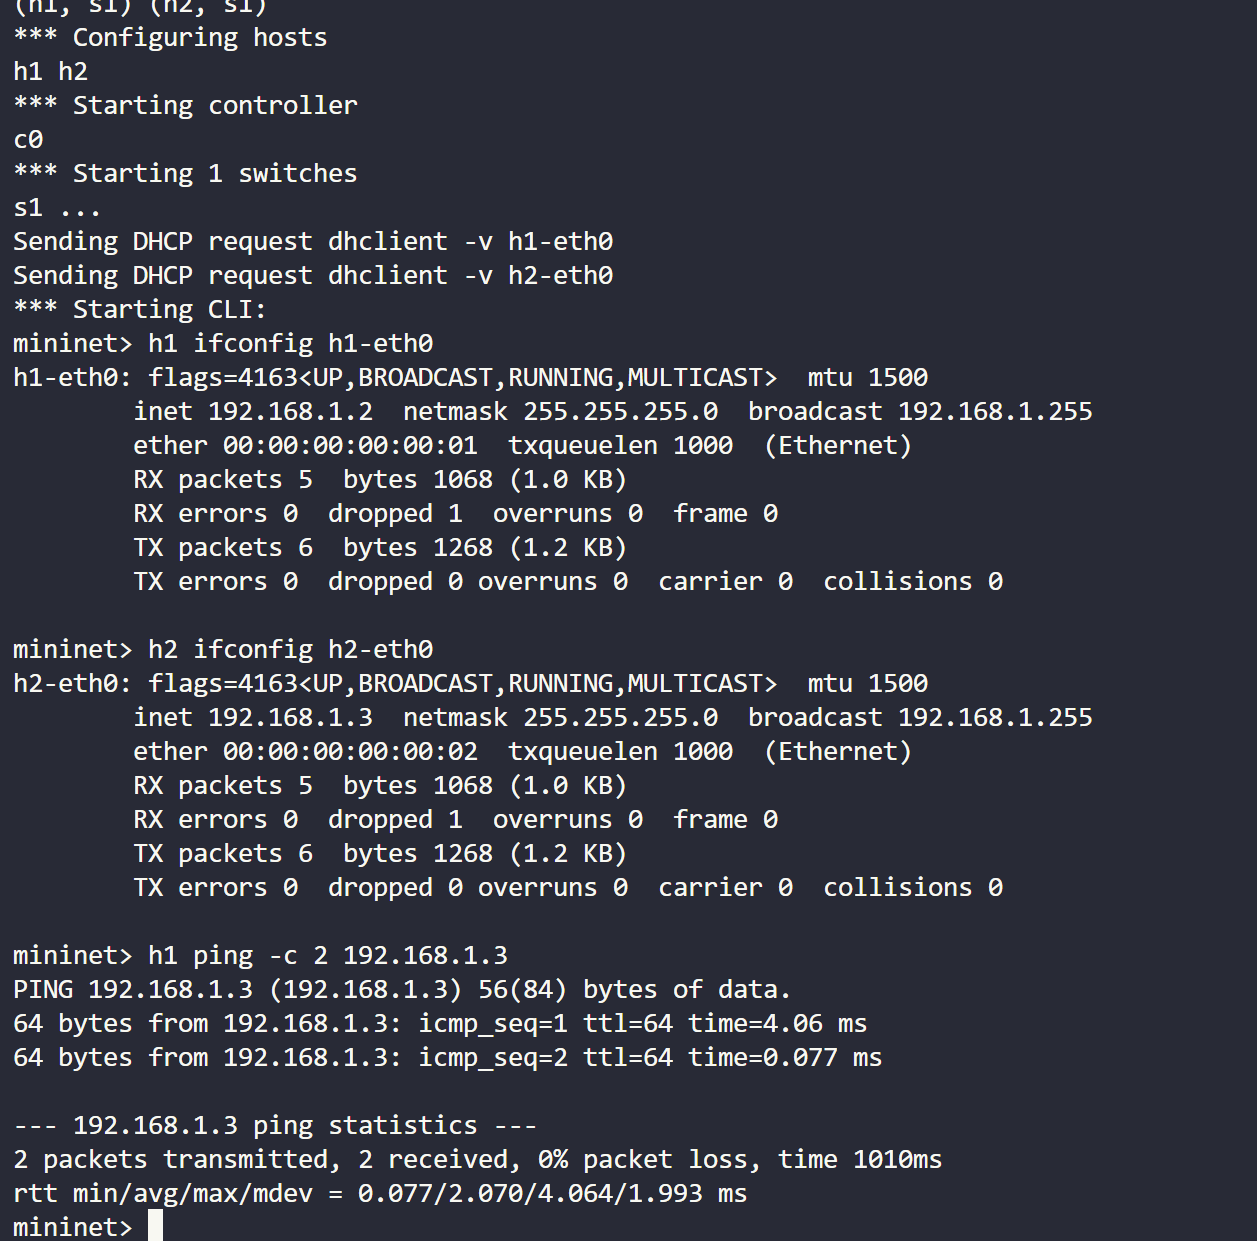
\includegraphics[width=0.62\textwidth]{img/dhcp_basic_result.png}
    \caption{基础 DHCP 测试结果，展示成功分配地址并完成连通性验证。}
\end{figure}

\begin{figure}[H]
    \centering
    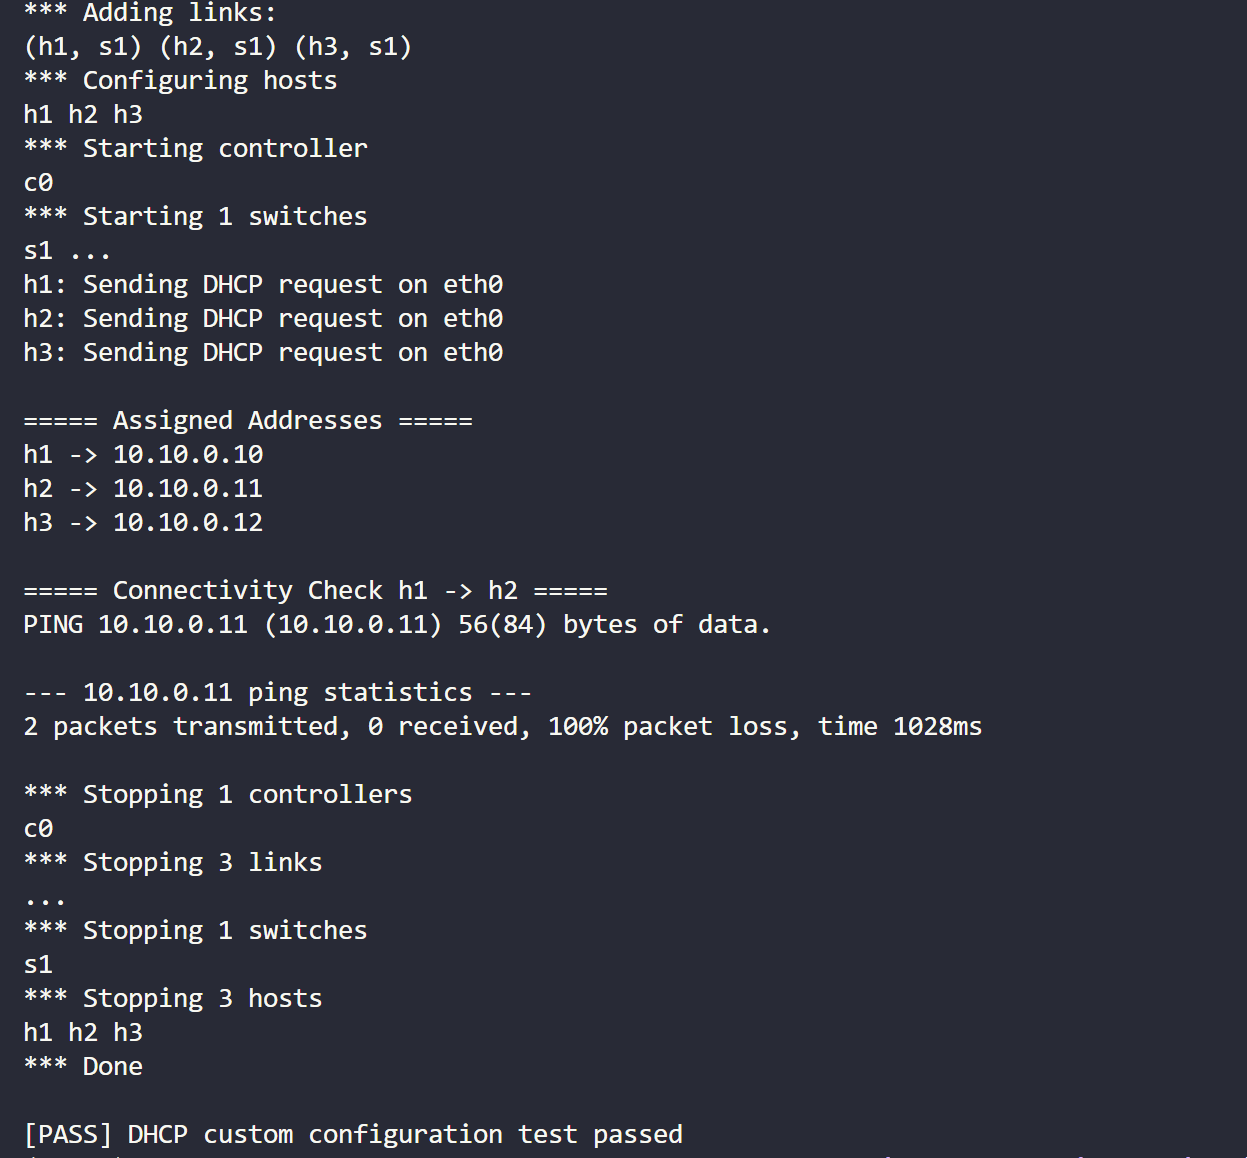
\includegraphics[width=0.62\textwidth]{img/dhcp_custom_result.png}
    \caption{自定义地址池与子网掩码下的 DHCP 测试结果。}
\end{figure}

\begin{figure}[H]
    \centering
    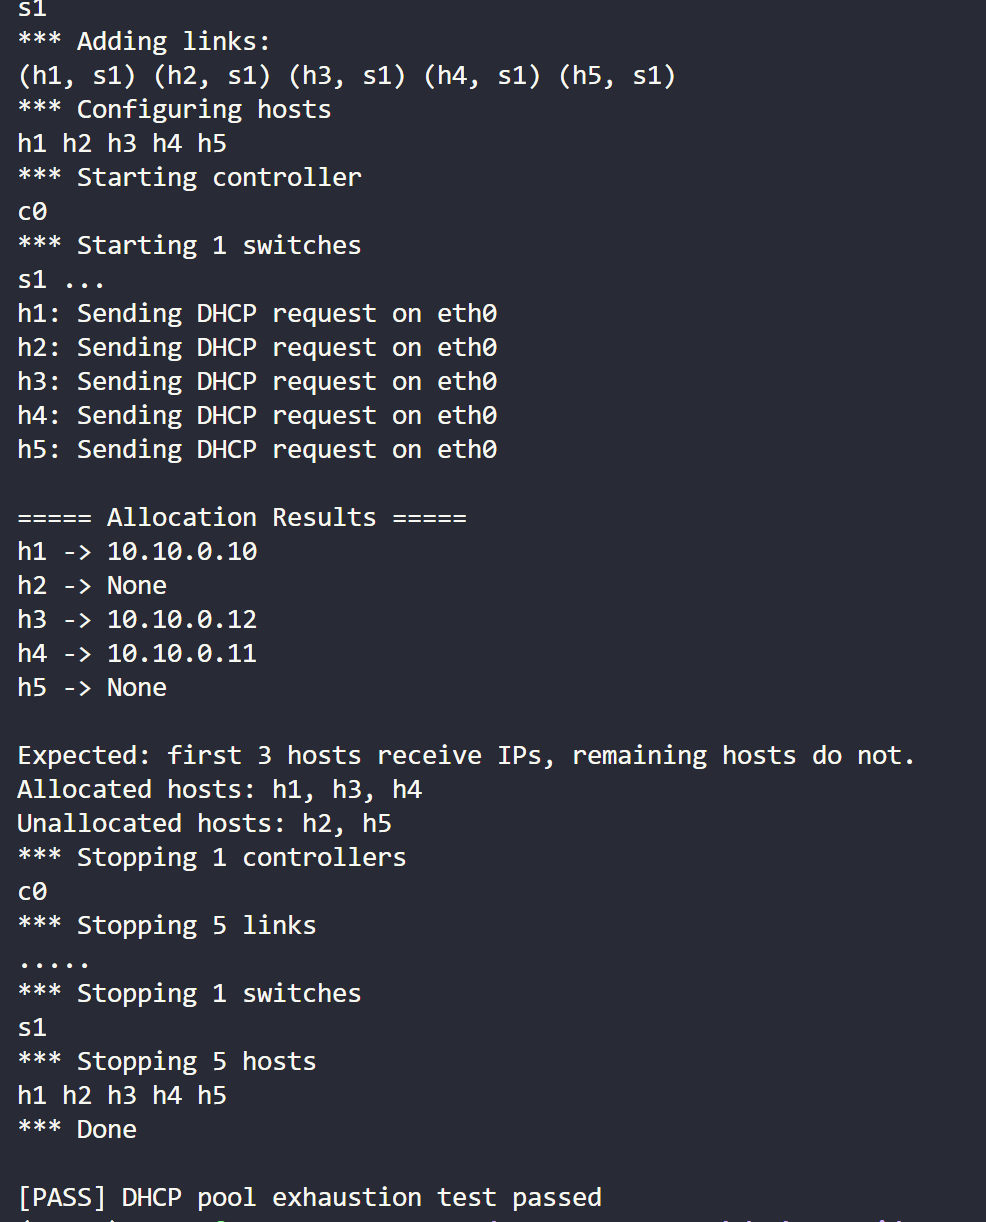
\includegraphics[width=0.55\textwidth]{img/dhcp_pool_exhaustion.png}
    \caption{地址池耗尽测试结果，只有前几个主机获得地址。}
\end{figure}

\subsection{Shortest-Path Switching Tests}

\begin{itemize}[leftmargin=1.5em]
    \item 基础三角拓扑下的全连通验证；
    \item 超过 6 台主机、6 台交换机、10 条边的复杂拓扑；
    \item 链路 down/up、交换机 stop/start、端口 disable/enable 等动态变化。
\end{itemize}

\begin{figure}[H]
    \centering
    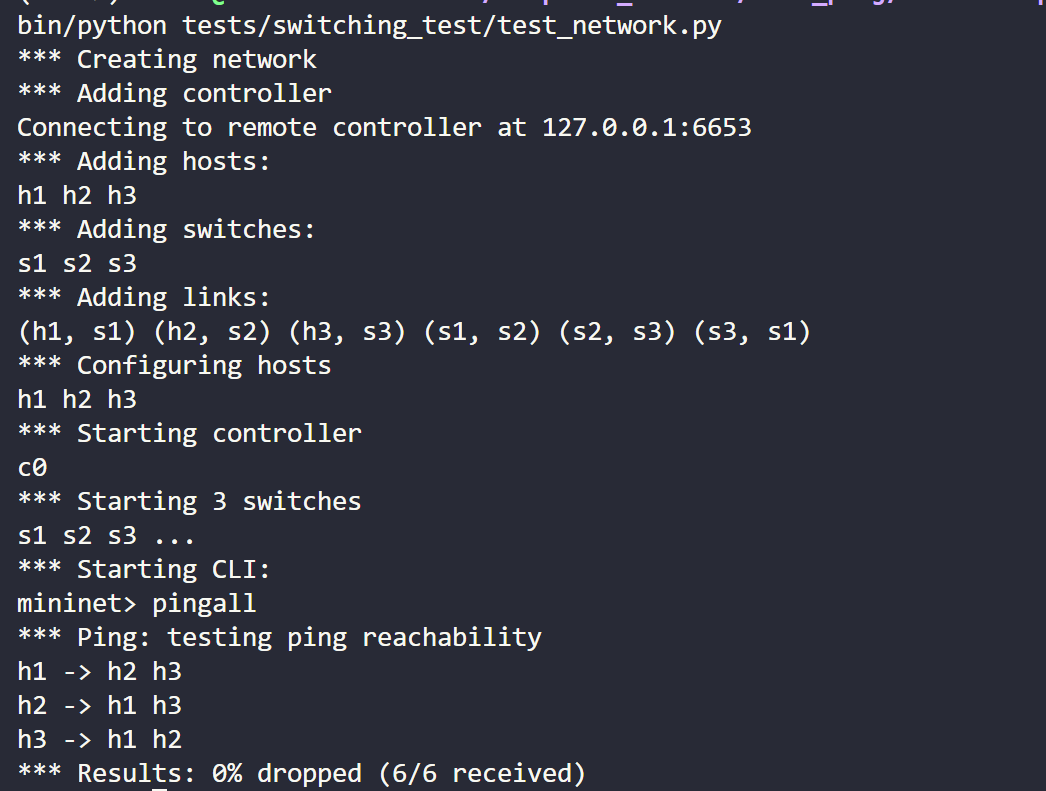
\includegraphics[width=0.56\textwidth]{img/switching_basic_pingall.png}
    \caption{基础三角拓扑中的交换与连通性验证。}
\end{figure}

\subsection{Firewall Tests}

\begin{itemize}[leftmargin=1.5em]
    \item 单交换机场景下的基础防火墙策略验证；
    \item 复用复杂交换拓扑的多交换机防火墙场景；
    \item 验证指定通信被阻断，而无关流量仍可正常通过。
\end{itemize}

\begin{figure}[H]
    \centering
    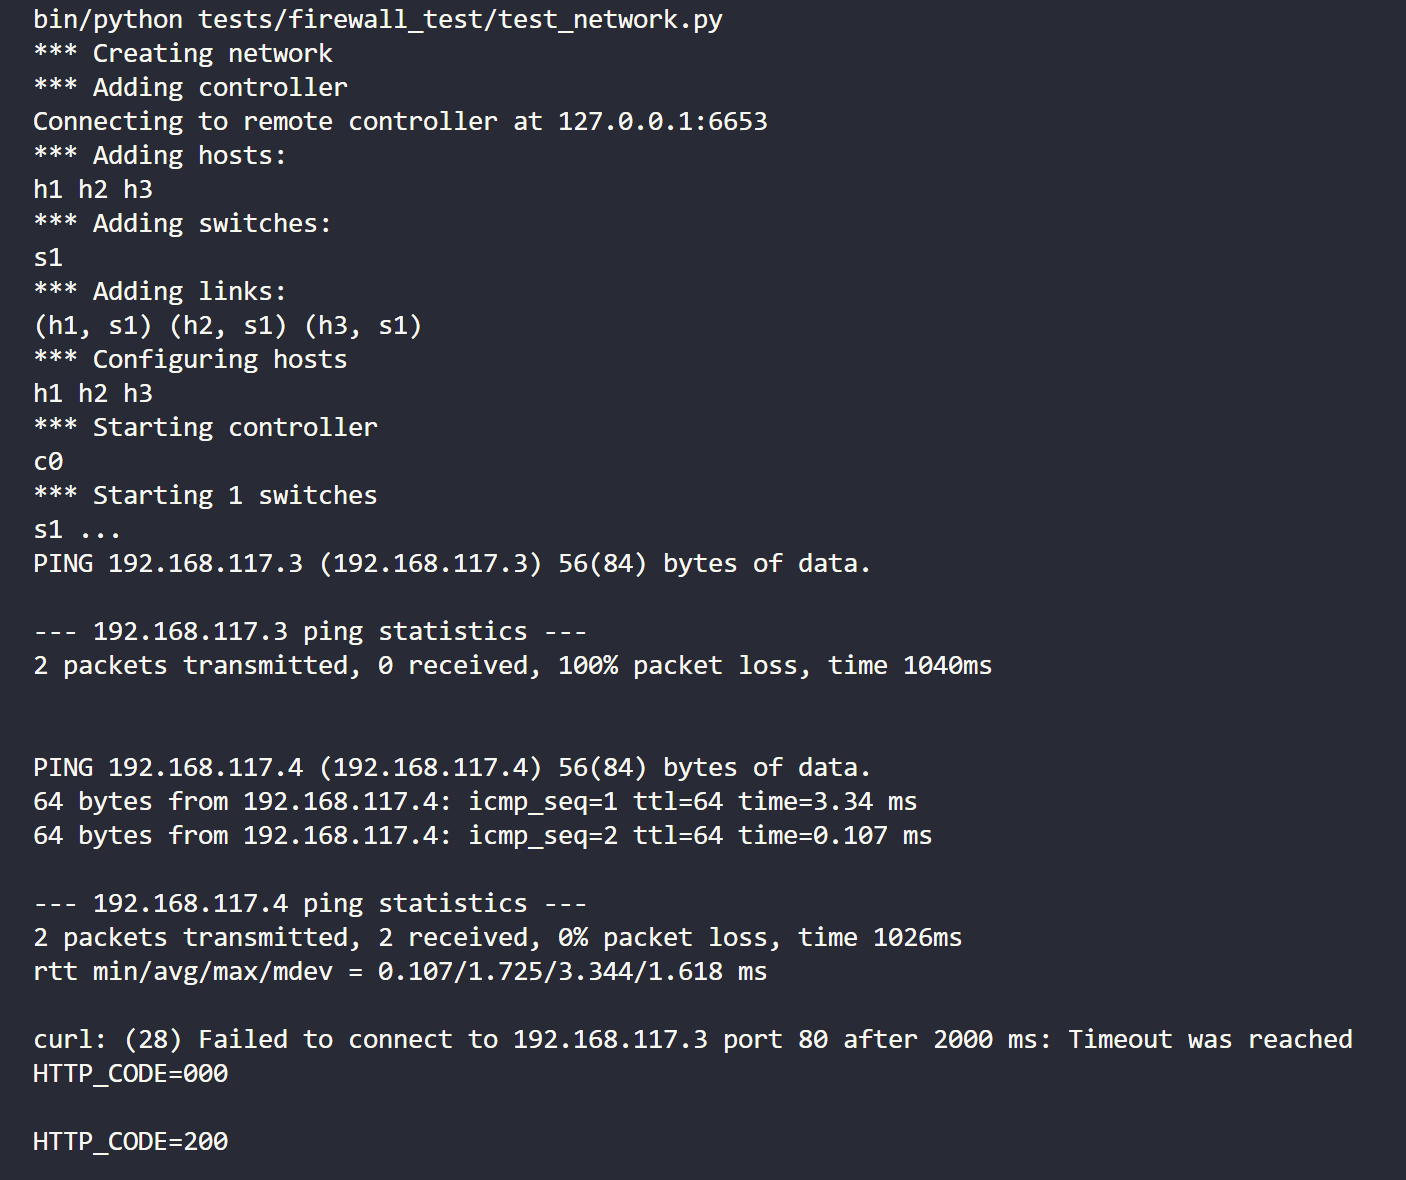
\includegraphics[width=0.78\textwidth]{img/firewall_basic.png}
    \caption{基础防火墙测试结果。}
\end{figure}

\begin{figure}[H]
    \centering
    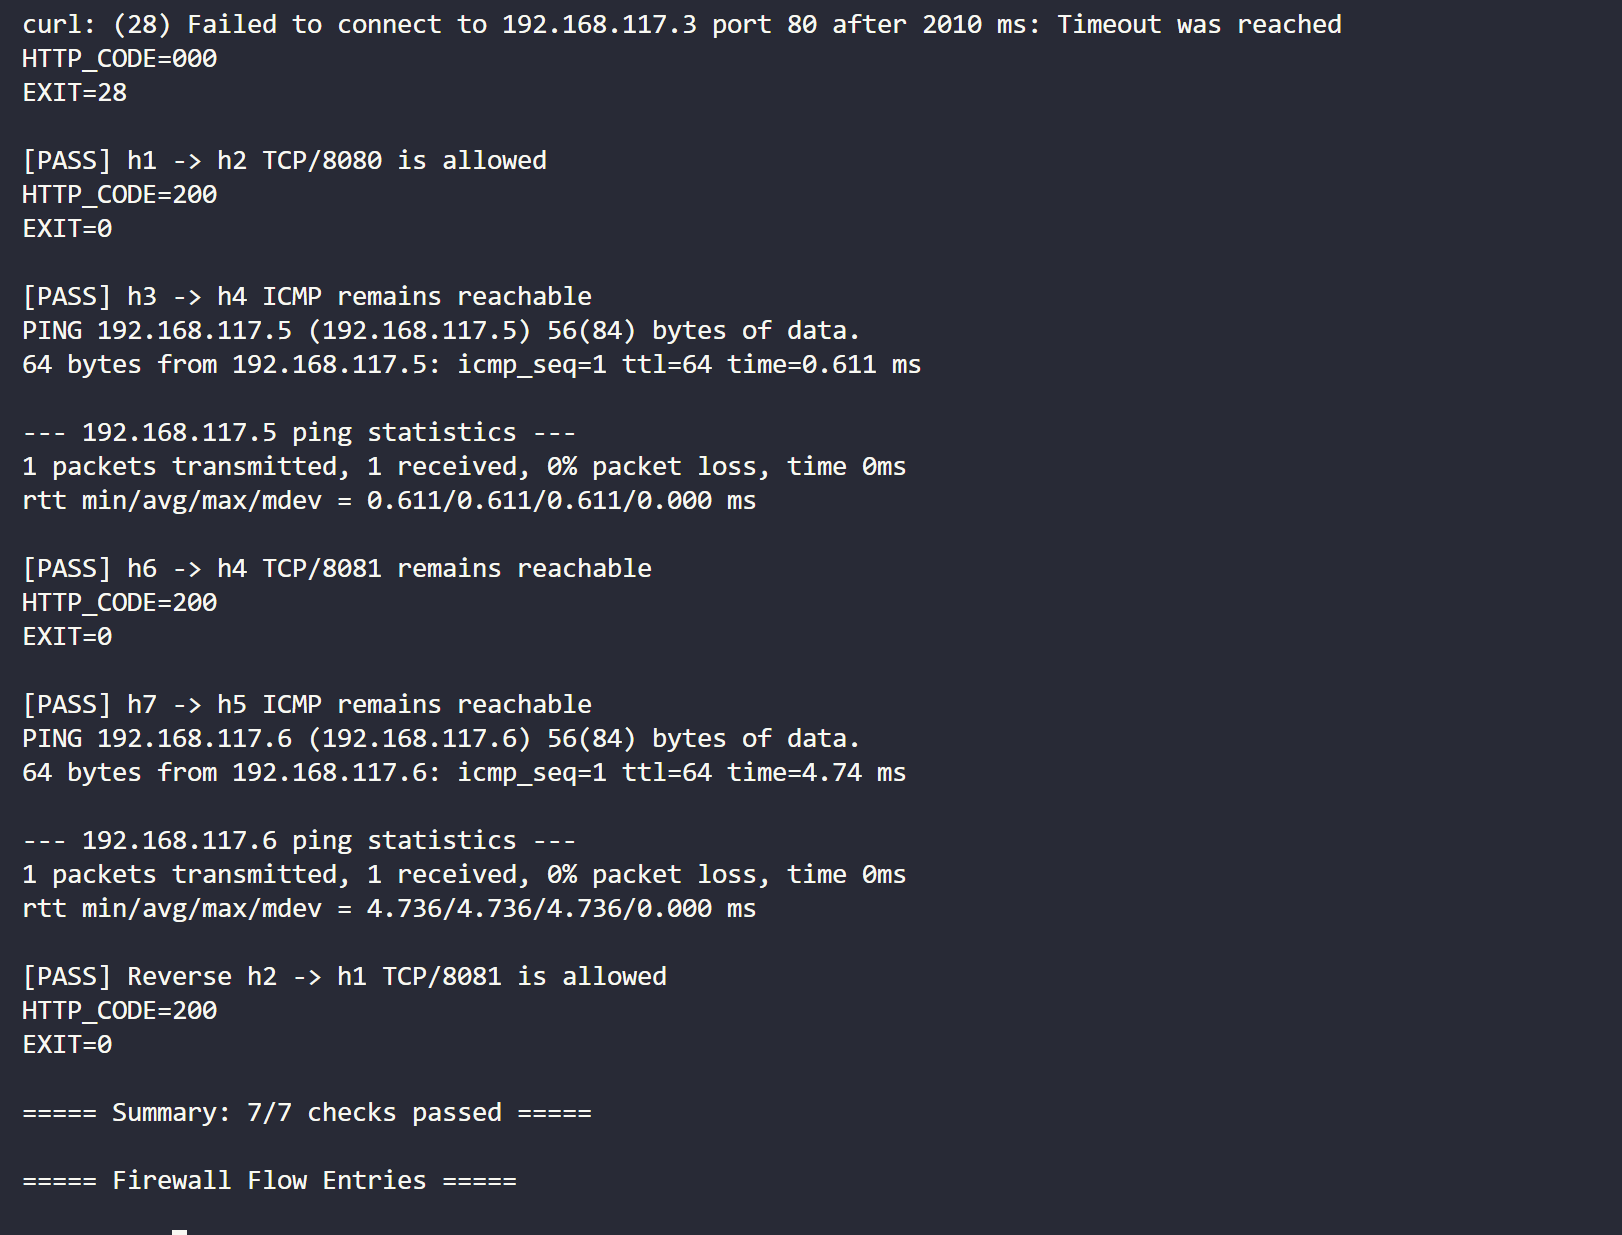
\includegraphics[width=0.72\textwidth]{img/firewall_complex_result.png}
    \caption{复杂拓扑下的防火墙测试结果。}
\end{figure}

\section{复杂测试案例}

项目要求设计一个超过 6 台主机、6 台交换机、10 条边的复杂拓扑。我们构建了符合要求的拓扑，并将其同时用于交换和防火墙部分的演示。

\subsection{拓扑概要}

\begin{itemize}[leftmargin=1.5em]
    \item Hosts: 7
    \item Switches: 7
    \item Inter-switch edges: 12
\end{itemize}

完整的 Mermaid 拓扑图与主机间最短路径表整理在 \texttt{docs/complex-case-topology.md} 中。

\begin{figure}[H]
    \centering
    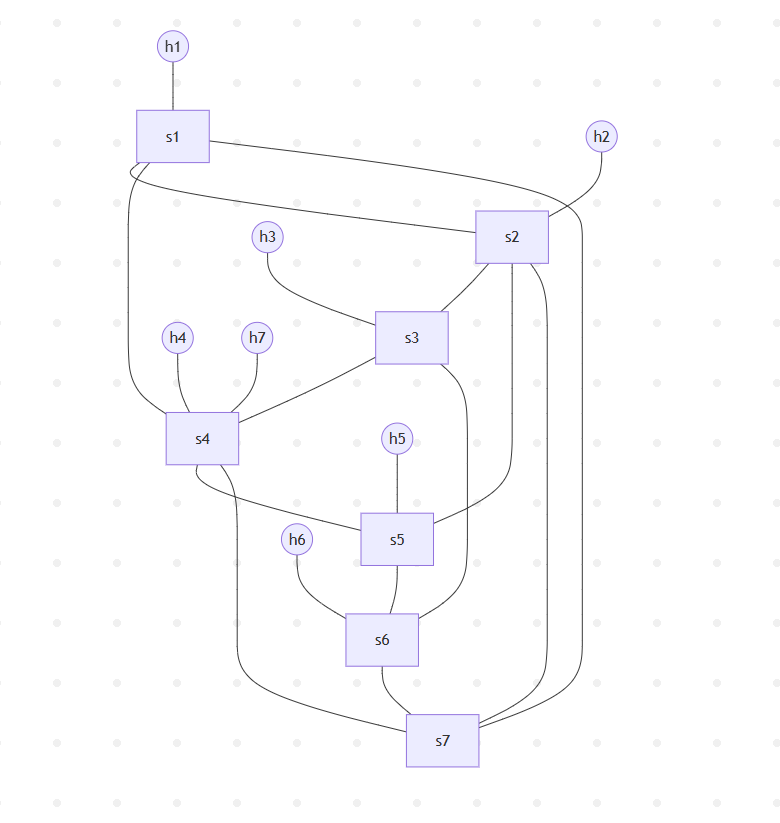
\includegraphics[width=0.42\textwidth]{img/switching_complex_topo.png}
    \caption{扩展演示中使用的复杂拓扑。}
\end{figure}

\subsection{动态操作}

该复杂案例支持以下 Mininet CLI 操作：

\begin{itemize}[leftmargin=1.5em]
    \item link down/up；
    \item switch stop/start；
    \item 通过 \texttt{ovs-ofctl mod-port} 进行 port down/up。
\end{itemize}

这些操作用于展示控制器在拓扑变化时重新计算路径并刷新流表的能力。

\begin{figure}[H]
    \centering
    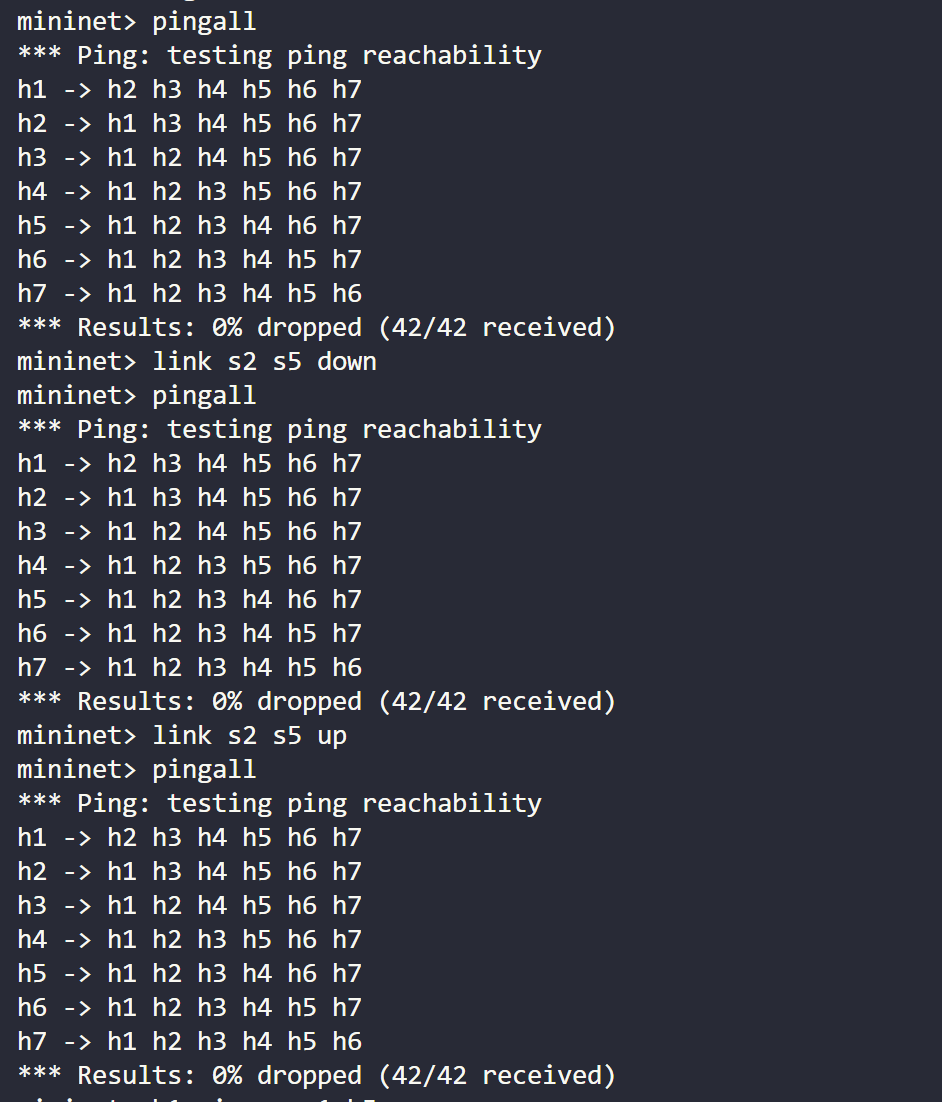
\includegraphics[width=0.55\textwidth]{img/switching_complex_controller_paths.png}
    \caption{复杂拓扑动态变化过程中的连通性验证结果。}
\end{figure}

\section{Bonus 结果与分析}

\subsection{DHCP Bonus}

DHCP bonus 的重点，是将基础地址分配器扩展为一个更完整的 DHCP 服务。服务器侧维护四类核心状态：pending offers、confirmed leases、lease expiration timestamps，以及被客户端拒绝、不得再次分配的地址。基于这几类状态，系统能够完成租约回收、续租与冲突处理。

\subsubsection{DHCP 状态机}

本实现遵循 RFC 2131 的客户端生命周期，而不是把 DHCP 简化成一次性的 DORA 交换。服务器能够区分正常的 \texttt{DISCOVER -> OFFER -> REQUEST -> ACK} 路径，以及 INIT-REBOOT、RENEWING、REBINDING 等不同类型的 REQUEST；同时，也支持显式的 RELEASE 与 DECLINE。因此，它实现的是租约管理逻辑，而不是一次性的地址发放。

\begin{figure}[H]
    \centering
    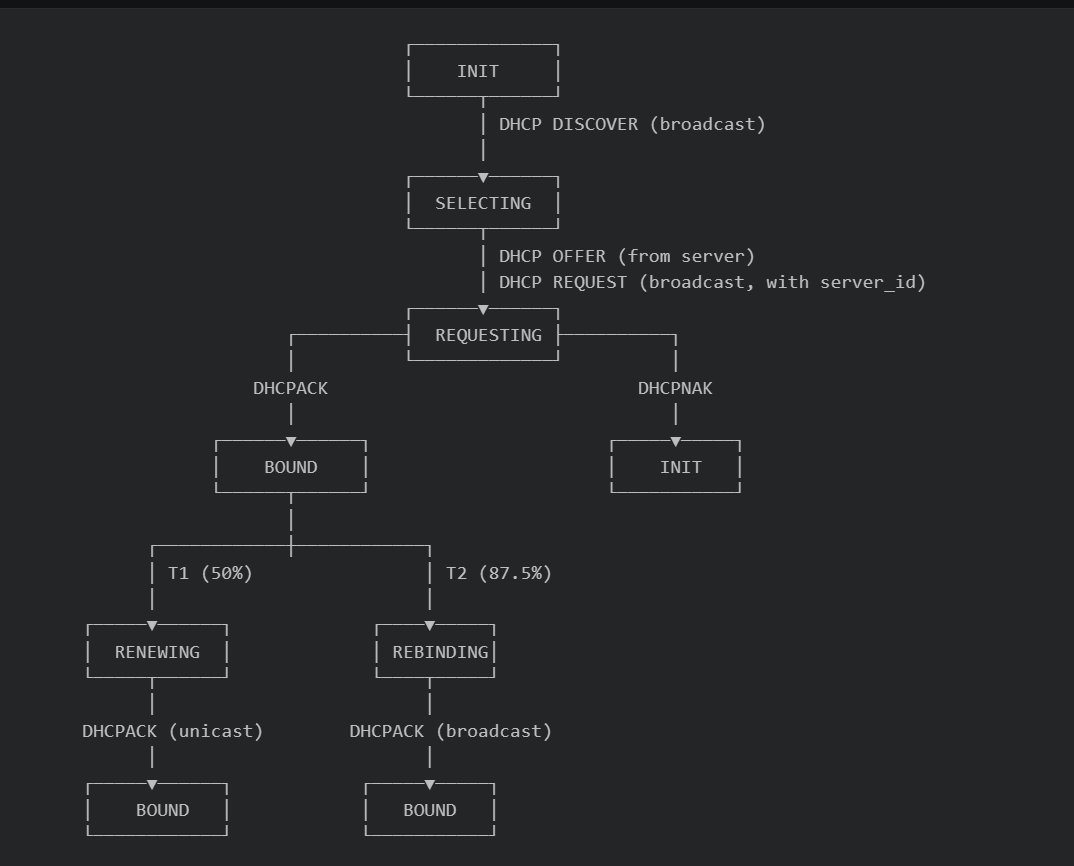
\includegraphics[width=0.82\textwidth]{img/dhcp_state.png}
    \caption{RFC 2131 中客户端 DHCP 状态迁移图，对应本实现中的租约管理逻辑。}
\end{figure}

该状态机在 \texttt{dhcp.py} 中有直接对应。REQUEST 处理逻辑不会把所有 REQUEST 一概而论，而是根据 \texttt{ciaddr}、Option 50 和 Option 54 识别语义，再执行不同的 RFC 处理路径。

\begin{lstlisting}[language=Python]
if ciaddr == '0.0.0.0' and requested_ip and server_id_opt:
    # SELECTING
    ...

if ciaddr == '0.0.0.0' and requested_ip and not server_id_opt:
    # INIT-REBOOT
    ...

if ciaddr and ciaddr != '0.0.0.0':
    # RENEWING / REBINDING
    ...
\end{lstlisting}

\subsubsection{Lease Expiration}

租约过期决定了地址何时能够在无人干预的情况下返回地址池。服务器为每个正式租约维护一个过期时间戳，并在当前时间超过该时间点后回收该租约。

\begin{lstlisting}[language=Python]
@classmethod
def _is_expired(cls, ip: str) -> bool:
    expiry = cls.lease_expiry.get(ip)
    return expiry is not None and time.time() > expiry

@classmethod
def _reclaim_expired(cls):
    now = time.time()

    expired_macs = [
        mac for mac, ip in cls.ip_pool.items()
        if cls._is_expired(ip)
    ]
    for mac in expired_macs:
        ip = cls.ip_pool.pop(mac)
        cls.lease_expiry.pop(ip, None)
\end{lstlisting}

在报告展示中，我们将“自然过期测试”作为这一部分的主示例。租期到达后，服务器侧旧租约被回收，客户端清空旧状态后重新发起请求，并再次获得可用租约。这个过程直接验证了过期与复用机制。

\begin{figure}[H]
    \centering
    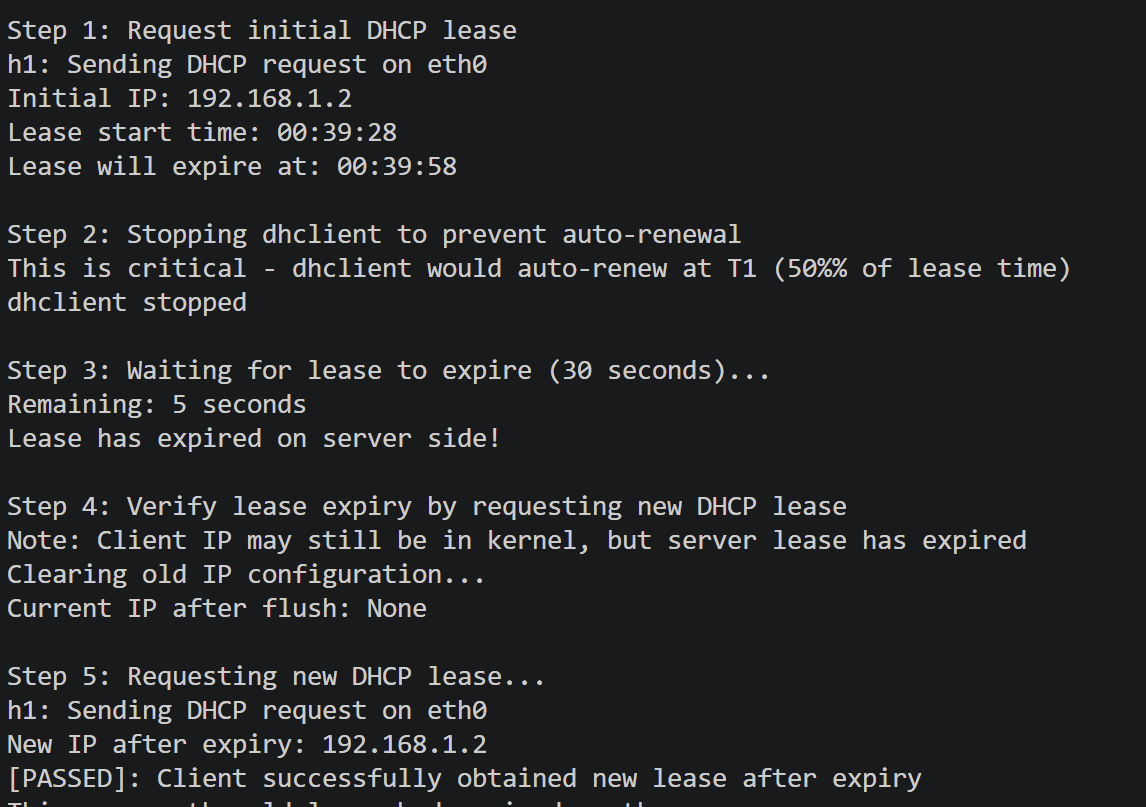
\includegraphics[width=0.82\textwidth]{img/lease_guoqi.png}
    \caption{租约过期测试：原租约在服务器侧自然失效，客户端清空旧配置后再次成功获取新租约。}
\end{figure}

\subsubsection{Duplicate-IP Prevention}

为了避免两个客户端获得同一个地址，分配器采用了原子 reservation 机制。它在分配新地址前会先回收过期资源，然后同时检查正式租约表与 pending-offer 表；一旦找到可用地址，就立即写入 \mbox{\texttt{pending\_offers}}。这样即使多个客户端在相近时间发送 DISCOVER，也不会观察到同一个空闲地址。

\begin{lstlisting}[language=Python]
@classmethod
def _allocate_ip(cls, client_mac: str) -> Optional[str]:
    cls._reclaim_expired()

    if client_mac in cls.ip_pool:
        return cls.ip_pool[client_mac]
    if client_mac in cls.pending_offers:
        return cls.pending_offers[client_mac]["ip"]

    in_use = cls._in_use_ips()
    for ip in cls._build_ip_range():
        if ip not in in_use and ip not in cls.bad_ips:
            cls.pending_offers[client_mac] = {
                "ip": ip,
                "timestamp": time.time(),
            }
            return ip
    return None
\end{lstlisting}

并发分配测试在开发过程中用于验证实现，但截图本身并不能像分配逻辑与日志那样直接说明“无重复 IP”这一性质。因此最终报告保留机制说明，而不再放入两张并发测试截图。

\subsubsection{OFFER Timeout Reclaim}

服务器也会清理过期的 \mbox{\texttt{pending\_offers}}。如果客户端收到了 OFFER，但没有继续发送 REQUEST 确认，那么这个 reservation 会在 \texttt{offer\_timeout} 秒后被释放，地址随之重新进入可分配状态。

\begin{lstlisting}[language=Python]
expired_offer_macs = [
    mac for mac, info in cls.pending_offers.items()
    if now - info["timestamp"] > cls.offer_timeout
]
for mac in expired_offer_macs:
    info = cls.pending_offers.pop(mac)
\end{lstlisting}

\begin{figure}[H]
    \centering
    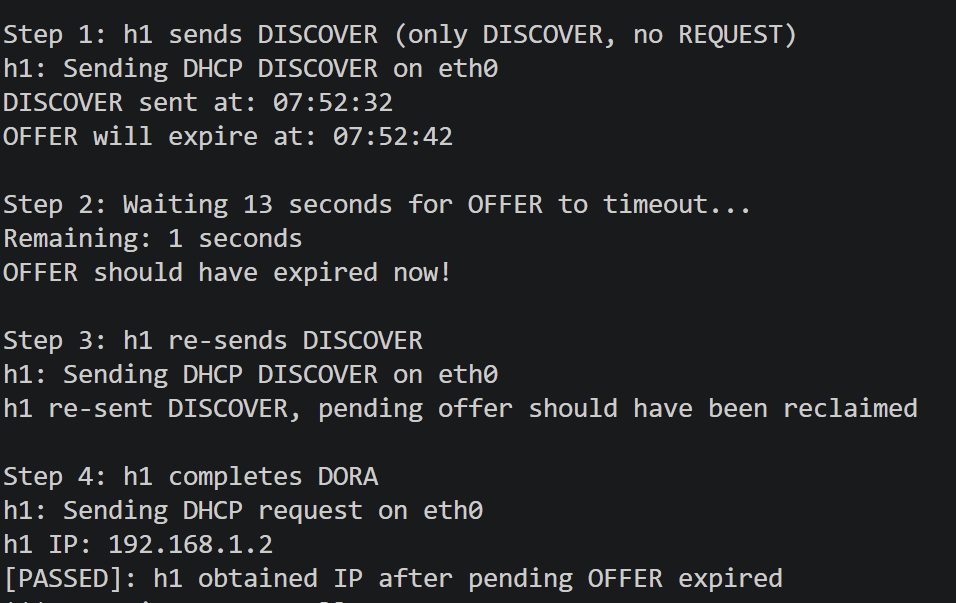
\includegraphics[width=0.72\textwidth]{img/dhcp_test3.png}
    \caption{DHCP OFFER 超时回收测试结果。}
\end{figure}

\subsubsection{Lease Renewal}

对于 RENEWING 和 REBINDING，客户端已经持有地址，因此服务器需要验证 \texttt{ciaddr} 是否确实仍属于当前 MAC，再延长租约时间。这样可以保证续租操作仍然绑定到正确的租约记录。

\begin{figure}[H]
    \centering
    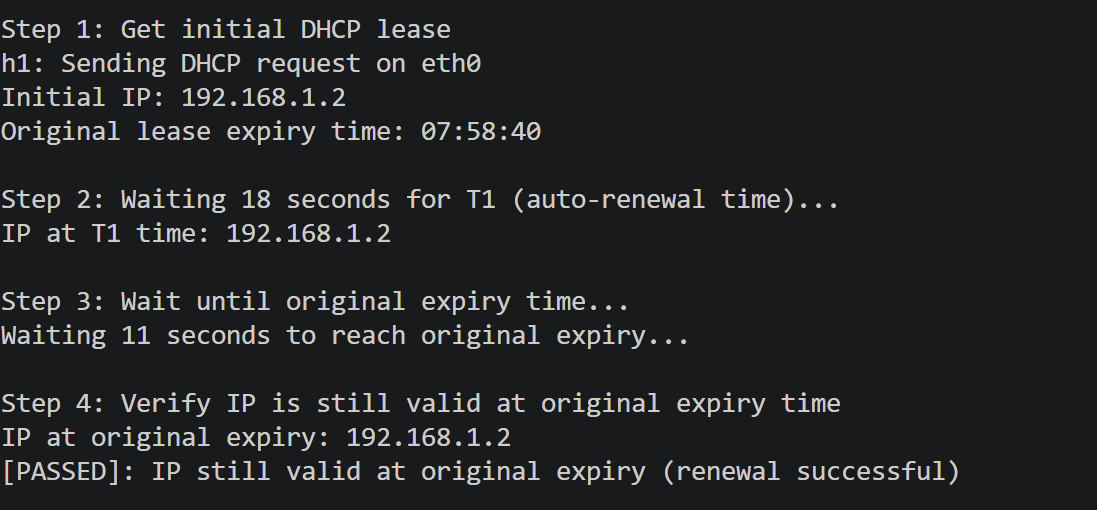
\includegraphics[width=0.72\textwidth]{img/dhcp_test2.png}
    \caption{租约续租测试：客户端在租约失效前完成续租，并保持原有地址。}
\end{figure}

\begin{lstlisting}[language=Python]
if ciaddr and ciaddr != '0.0.0.0':
    existing_ip = cls.ip_pool.get(client_mac)
    if existing_ip != ciaddr:
        return cls._build_nak_pkt(client_mac, xid)
    if cls._is_expired(ciaddr):
        cls.ip_pool.pop(client_mac, None)
        cls.lease_expiry.pop(ciaddr, None)
        return cls._build_nak_pkt(client_mac, xid)

    cls.lease_expiry[ciaddr] = time.time() + cls.lease_time
    return cls._build_reply_pkt(
        client_mac, xid, ciaddr, dhcp.DHCP_ACK,
        unicast_ip=ciaddr
    )
\end{lstlisting}

\subsubsection{DHCPNAK Handling}

对于非法或不一致的请求，服务器会构造 RFC 兼容的 DHCPNAK。特别地，返回报文中的 \texttt{yiaddr} 为 \texttt{0.0.0.0}，并且通过广播发送，因为客户端在该时刻可能并不持有可用地址。

\begin{lstlisting}[language=Python]
@classmethod
def _build_nak_pkt(cls, client_mac: str, xid: int) -> packet.Packet:
    dhcp_pkt = dhcp.dhcp(
        op=dhcp.DHCP_BOOT_REPLY,
        chaddr=client_mac,
        siaddr=cls._gateway_ip,
        yiaddr='0.0.0.0',
        xid=xid,
        boot_file='',
        options=options,
    )
\end{lstlisting}

\subsubsection{DECLINE and RELEASE}

实现中还支持客户端主动释放租约以及上报地址冲突。RELEASE 会立即把地址归还给地址池；DECLINE 会将该地址从当前状态表中移除，并加入 \mbox{\texttt{bad\_ips}}，从而避免冲突地址再次被分配。

\begin{lstlisting}[language=Python]
@classmethod
def _handle_release(cls, pkt):
    ip = cls.ip_pool.pop(client_mac, None)
    if ip:
        cls.lease_expiry.pop(ip, None)
    cls.pending_offers.pop(client_mac, None)

@classmethod
def _handle_decline(cls, pkt):
    ...
    cls.bad_ips.add(declined_ip)
\end{lstlisting}

\subsubsection{Broadcast and Unicast Reply Selection}

回复路径明确区分了“初始化阶段”和“续租阶段”。对于尚未获得地址的客户端，OFFER 和初始 ACK 采用广播回复；而对于已经持有地址的续租场景，则可以单播 ACK 到客户端现有地址。

\begin{lstlisting}[language=Python]
use_broadcast = unicast_ip is None
dst_mac = 'ff:ff:ff:ff:ff:ff' if use_broadcast else client_mac
dst_ip  = '255.255.255.255' if use_broadcast else unicast_ip
\end{lstlisting}

\subsection{DNS Bonus}

DNS bonus 展示了控制器不仅能做转发和 DHCP，也能充当一个简化版 DNS responder。

该实现完全位于控制器侧。启动时会从静态 JSON 文件读取 DNS server 的虚拟 IP、虚拟 MAC 以及域名到 IP 的映射表。当交换机加入时，控制器会安装一条高优先级的 PacketIn 规则，匹配 IPv4 UDP 53 端口，从而把 DNS 请求送到 controller，而不是走普通的最短路径转发。同时，控制器还会对虚拟 DNS IP \texttt{192.168.1.1} 的 ARP 请求进行应答，保证主机能够向这个“虚拟 DNS server”发出 UDP 报文。

DNS 响应路径实现在 \texttt{dns\_server.py} 中。控制器从 UDP payload 中取出 DNS query，解析 question，查静态记录表，然后手工构造完整的 DNS response 以太网帧，并通过 PacketOut 返回给请求主机。

\begin{lstlisting}[language=Python]
def install_packetin_flow(self, datapath, ofctl, ether_types, inet, vlan_id):
    actions = [
        datapath.ofproto_parser.OFPActionOutput(
            datapath.ofproto.OFPP_CONTROLLER,
            0xFFFF,
        )
    ]
    ofctl.set_flow(
        cookie=self.COOKIE,
        priority=self.PACKETIN_PRIORITY,
        dl_type=ether_types.ETH_TYPE_IP,
        dl_vlan=vlan_id,
        nw_proto=inet.IPPROTO_UDP,
        tp_dst=self.DNS_PORT,
        actions=actions,
    )
\end{lstlisting}

\begin{lstlisting}[language=Python]
def build_response(self, query):
    query_id, flags, qdcount, _, _, _ = struct.unpack("!HHHHHH", query[:12])
    question_end, qname = self._read_qname(query, 12)
    question = query[12:question_end + 4]
    qtype, qclass = struct.unpack("!HH", query[question_end:question_end + 4])
    answer_ip = self.records.get(self._normalize_name(qname))

    answer = b""
    rcode = 0
    if qtype == 1 and qclass == 1 and answer_ip:
        answer = self._build_a_answer(answer_ip)
    elif qtype == 1 and qclass == 1:
        rcode = 3

    response_flags = 0x8000 | 0x0400 | (flags & 0x0100) | rcode
    header = struct.pack("!HHHHHH", query_id, response_flags, 1, 1 if answer else 0, 0, 0)
    return header + question + answer
\end{lstlisting}

测试拓扑为简单的 \texttt{h1-s1-h2} 场景。测试脚本验证三件事：
\texttt{web.cs305.local} 能否解析为 \texttt{192.168.1.3}，
\texttt{h1.cs305.local} 能否解析为 \texttt{192.168.1.2}，
以及不存在的域名能否返回 \texttt{NXDOMAIN}。此外，脚本还调用 \texttt{pingAll()} 验证 DNS 扩展没有破坏普通转发，并打印交换机流表，确认 UDP/53 的 PacketIn 规则确实存在。

\begin{figure}[H]
    \centering
    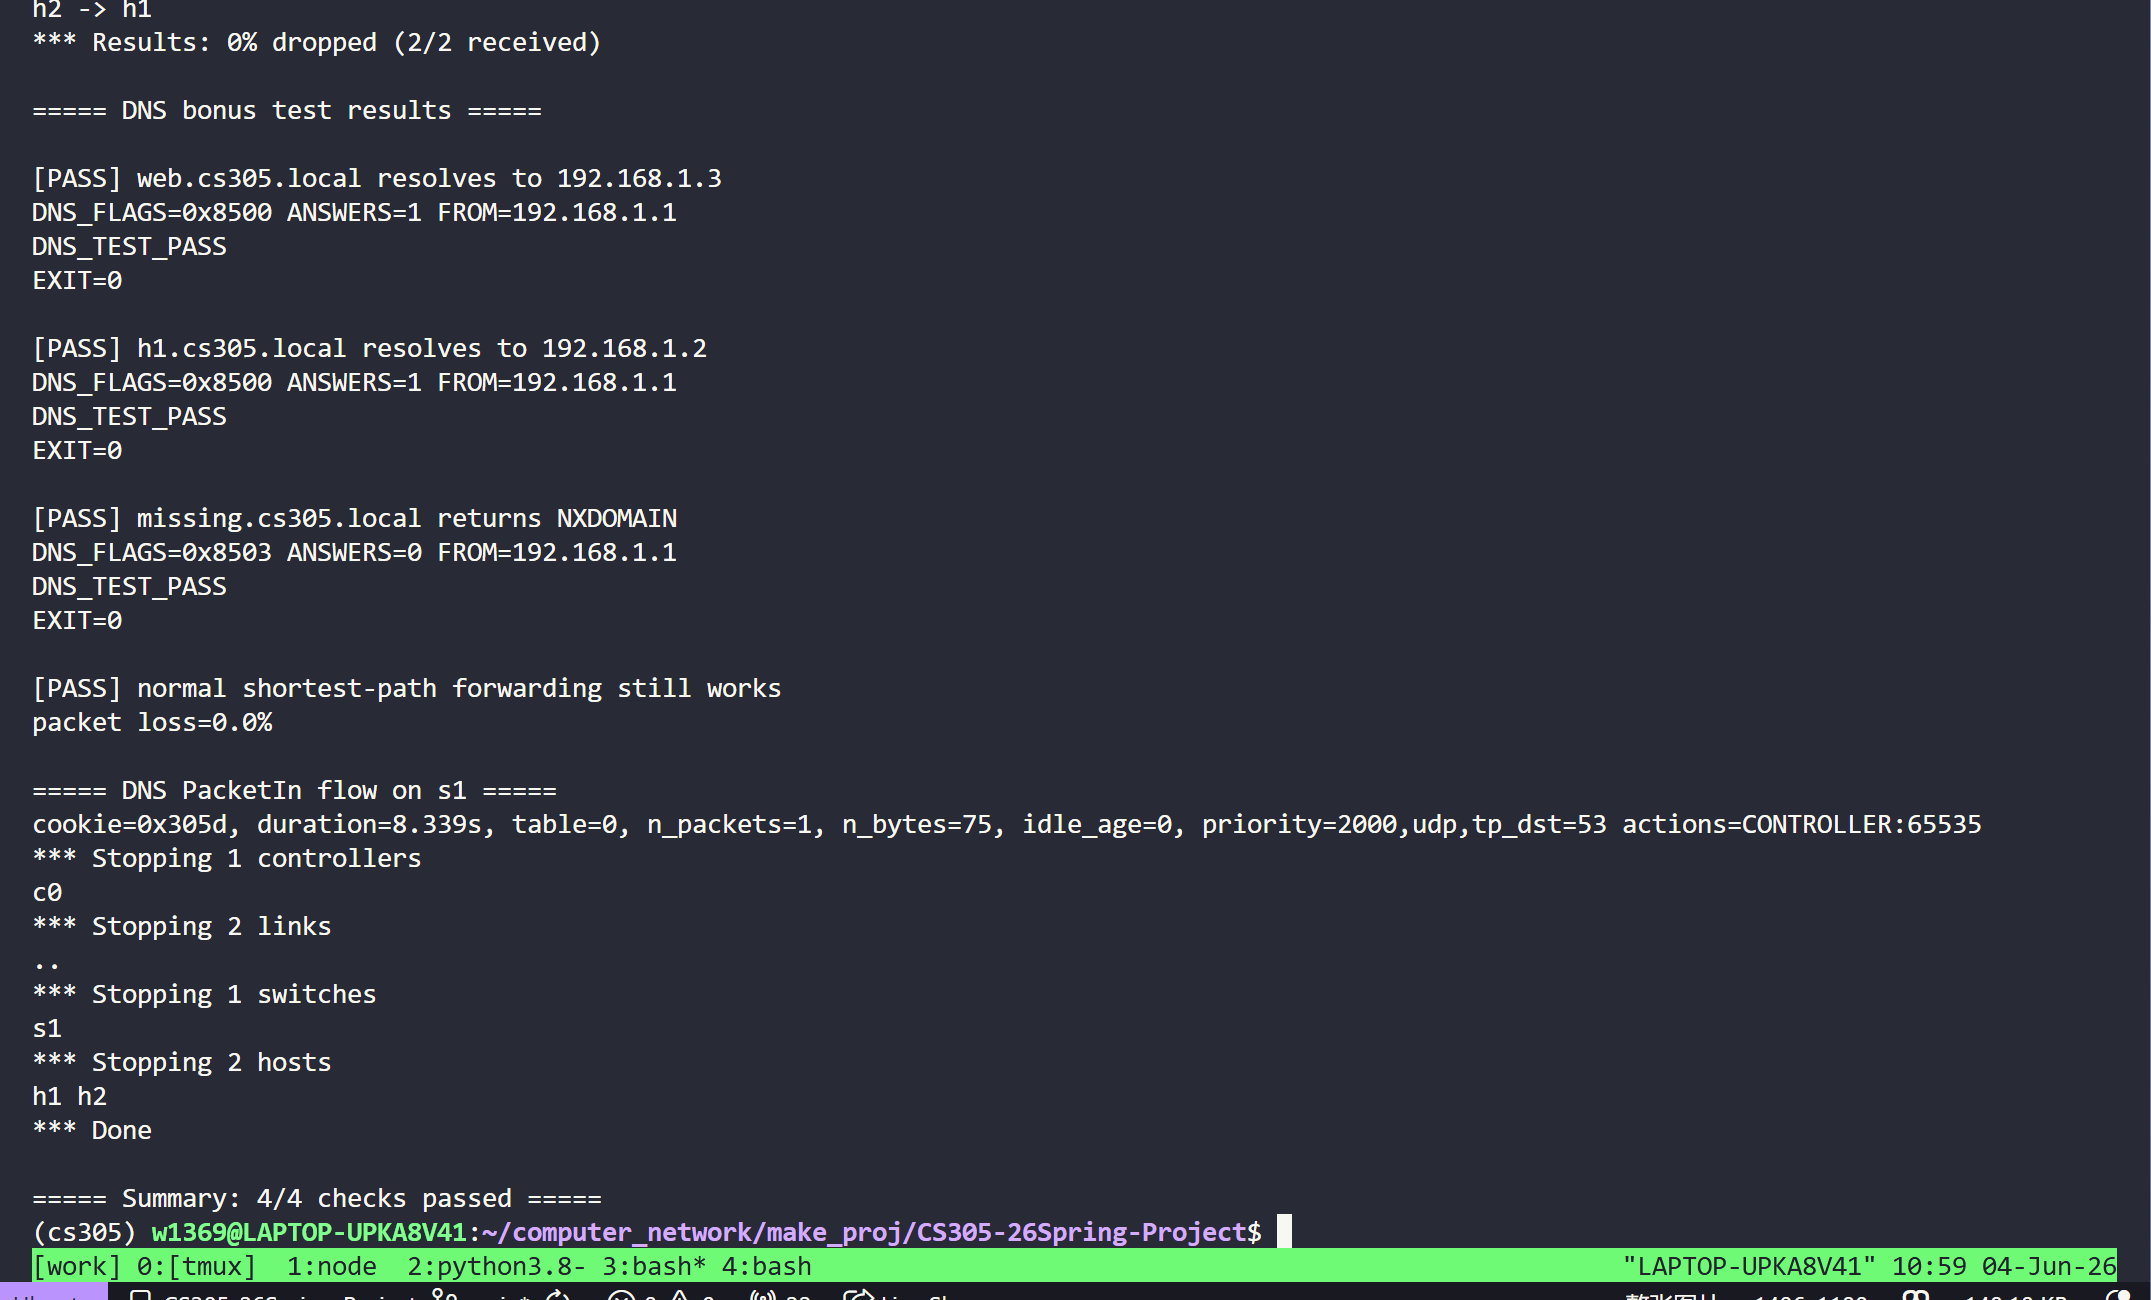
\includegraphics[width=0.78\textwidth]{img/dns_test.png}
    \caption{DNS bonus 测试结果。}
\end{figure}

\subsection{TCP Congestion Bonus}

TCP congestion bonus 用于比较不同拥塞控制算法在相同瓶颈链路上的行为差异。实验结果表明，不同算法会带来不同的吞吐表现，而在双流共享瓶颈时，fairness 通常仍然接近 1。

这一 bonus 是 Mininet 实验，而不是控制器内功能。拓扑中包含四台主机和两台交换机，\texttt{s1} 与 \texttt{s2} 之间有一条唯一瓶颈链路。接入链路配置为 \texttt{100 Mbps, 1 ms}，瓶颈链路配置为 \texttt{10 Mbps, 30 ms, 0.5\% loss, queue size 100}。其中 \texttt{0.5\%} 的随机丢包由 \texttt{TCLink} 直接设置，用于构造一个可控的拥塞信号环境，以观察 Reno 和 CUBIC 在丢包后的恢复差异。

脚本包含两类实验。第一类是单流实验：\texttt{h1 -> h2} 分别在 Reno 和 CUBIC 下各运行一次。第二类是公平性实验：\texttt{h1 -> h2} 使用 Reno，\texttt{h3 -> h4} 使用 CUBIC，同时共享同一条瓶颈链路。吞吐量通过 \texttt{iperf} 输出解析，公平性通过 Jain's fairness index 计算。

\begin{lstlisting}[language=Python]
def set_tcp_algorithm(host, algorithm):
    host.cmd("modprobe tcp_%s 2>/dev/null || true" % algorithm)
    output = host.cmd(
        "sysctl -w net.ipv4.tcp_congestion_control=%s 2>&1" % algorithm
    )
    current = host.cmd("sysctl -n net.ipv4.tcp_congestion_control 2>/dev/null").strip()
    if current != algorithm:
        return False
    return True
\end{lstlisting}

\begin{lstlisting}[language=Python]
def jain_fairness(x1, x2):
    if x1 is None or x2 is None:
        return None
    denominator = 2 * (x1 ** 2 + x2 ** 2)
    if denominator == 0:
        return None
    return (x1 + x2) ** 2 / denominator
\end{lstlisting}

从定性预期来看，CUBIC 在单流场景下通常会比 Reno 有更高的平均吞吐量，因为它在丢包后的窗口恢复更积极；与此同时，公平性实验的结果一般仍会接近 1，说明两条流即使采用不同算法，也能在瓶颈链路上较为均衡地共享带宽。我们多次实验的结果也符合这一趋势：CUBIC 的平均单流吞吐量更高，而整体 fairness 保持较高水平。

\begin{figure}[H]
    \centering
    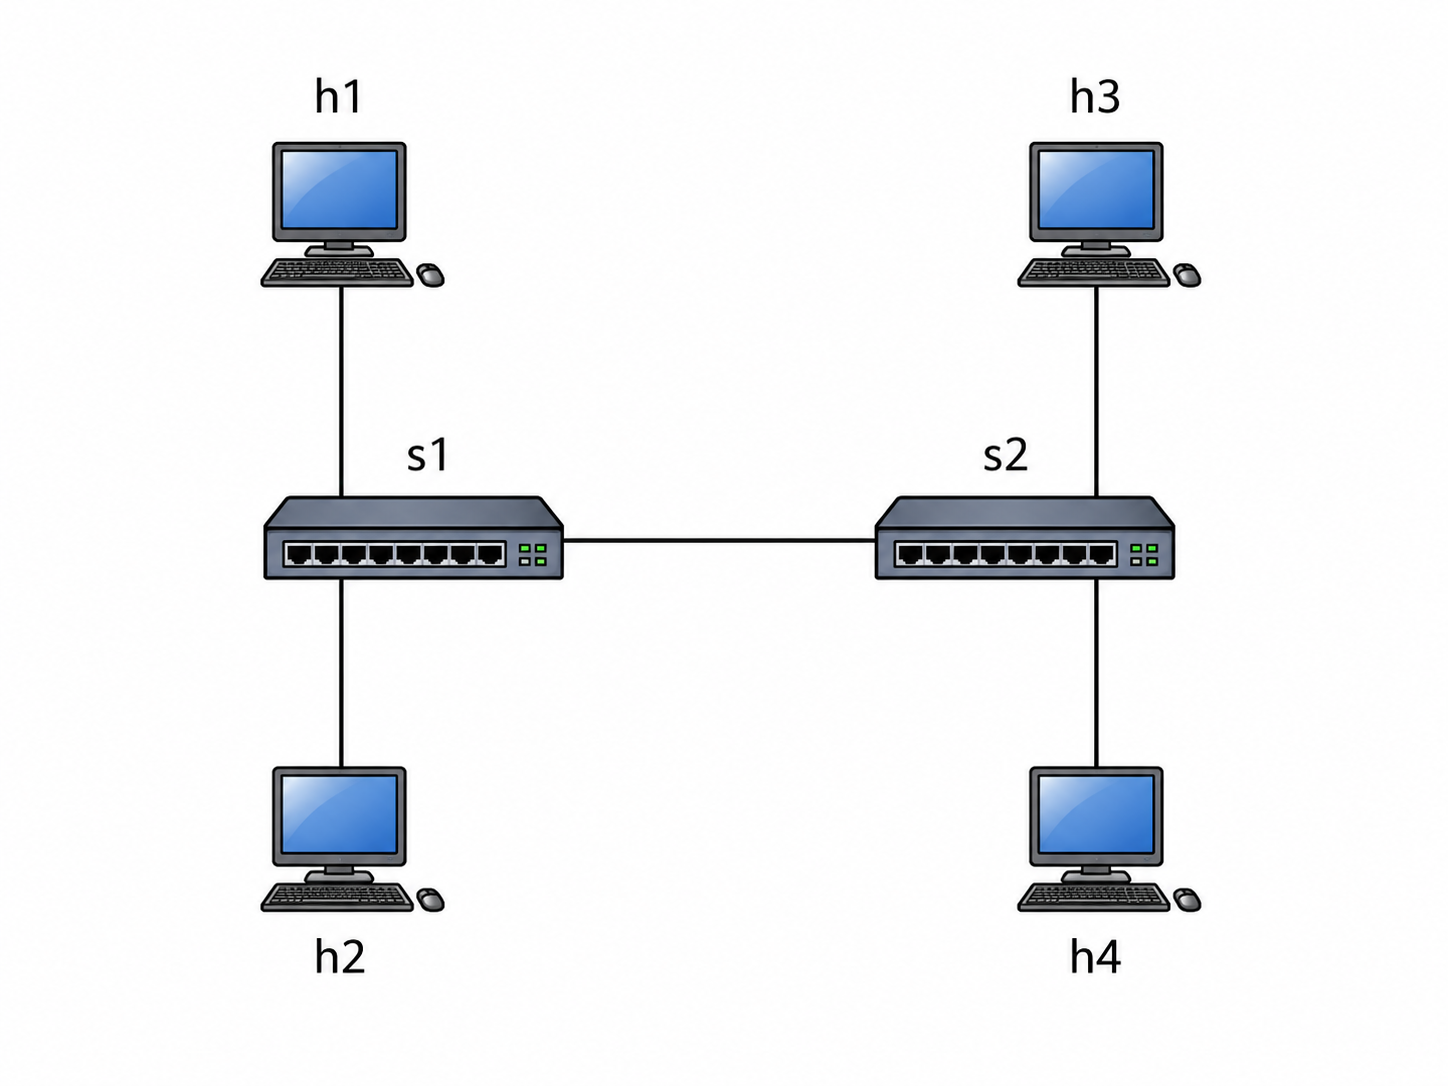
\includegraphics[width=0.72\textwidth]{img/bonus5_topo.png}
    \caption{TCP congestion 与 bufferbloat bonus 共用的 Mininet 实验拓扑。}
\end{figure}

\begin{figure}[H]
    \centering
    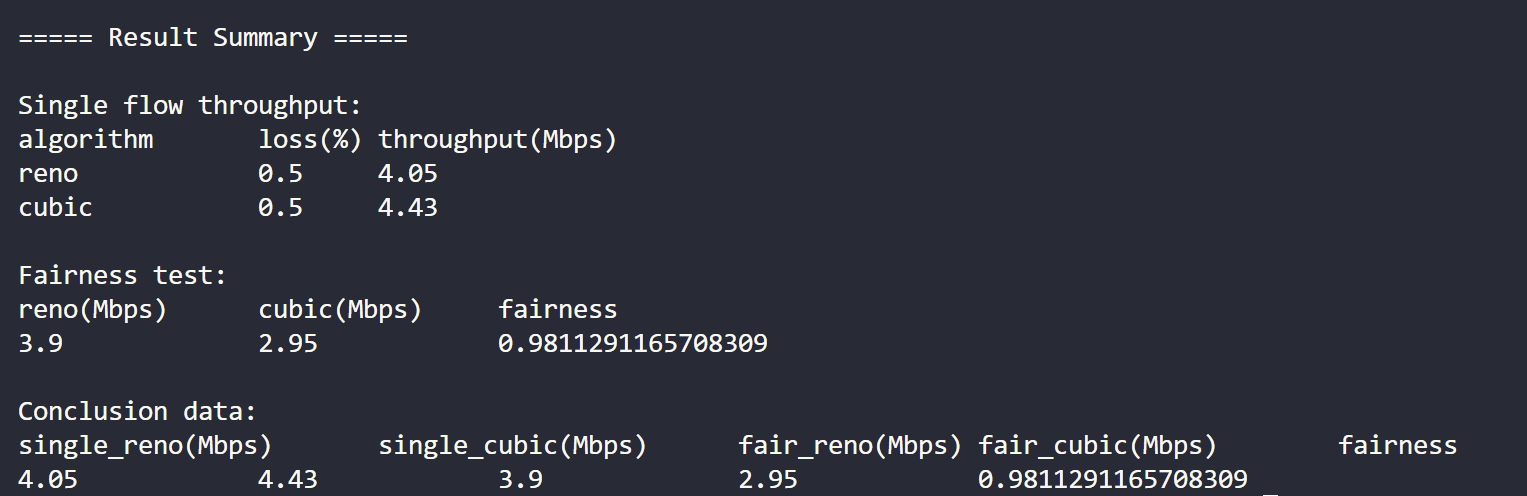
\includegraphics[width=0.82\textwidth]{img/tcp_congestion.png}
    \caption{Reno、CUBIC 以及 fairness 测试的 TCP congestion 实验结果。}
\end{figure}

\subsection{Bufferbloat Bonus}

Bufferbloat 实验展示了经典的吞吐量与时延权衡：当队列非常大时，丢包率可以下降，TCP 吞吐量也可能上升，但在有大流量时，交互流量的 RTT 会显著膨胀。

该实验沿用两台交换机的基本结构，但修改了瓶颈链路配置。接入链路保持为 \texttt{100 Mbps, 1 ms}，而 \texttt{s1-s2} 的瓶颈链路设置为 \texttt{1 Mbps, 20 ms}。实验中唯一变化的参数是瓶颈队列大小：一组使用 \texttt{20 packets}，另一组使用 \texttt{1000 packets}。

实验同时运行两类流量：\texttt{h1 -> h3} 使用 \texttt{iperf} 产生长时间 TCP 大流量，\texttt{h2 -> h4} 使用 \texttt{ping} 作为交互式小包探测流。脚本先测量空闲状态下的 RTT baseline，然后启动后台 ping，再启动前台 TCP 大流，最后分别解析 \texttt{iperf} 输出和 ping 统计结果。

\begin{lstlisting}[language=Python]
def parse_ping(output):
    loss_match = re.search(r"(\d+(?:\.\d+)?)% packet loss", output)
    rtt_match = re.search(
        r"(?:rtt|round-trip) min/avg/max/(?:mdev|stddev) = "
        r"[\d.]+/([\d.]+)/[\d.]+/[\d.]+",
        output,
    )
    loss = float(loss_match.group(1)) if loss_match else None
    avg_rtt = float(rtt_match.group(1)) if rtt_match else None
    return loss, avg_rtt
\end{lstlisting}

\begin{lstlisting}[language=Python]
idle_ping = ping(h2, h4.IP())
idle_loss, idle_rtt = parse_ping(idle_ping)
h3.cmd("iperf -s -p 5001 >/tmp/bonus5_iperf_server.log 2>&1 &")
h2.cmd("ping -c 30 -i 0.5 -W 2 %s >/tmp/bonus5_ping.log 2>&1 &" % h4.IP())
iperf_output = h1.cmd("iperf -c %s -p 5001 -t %s" % (h3.IP(), duration))
busy_ping = h2.cmd("cat /tmp/bonus5_ping.log")
busy_loss, busy_rtt = parse_ping(busy_ping)
throughput = parse_iperf(iperf_output)
\end{lstlisting}

这一实验的预期结果，就是典型的 bufferbloat 现象：大队列会减少早期丢包，也可能提升 TCP 吞吐量，因为更多数据包被缓存而不是直接丢弃；但与此同时，小包交互流量必须排在大流量后面等待，因此 busy RTT 会非常明显地上升。我们的实验结果也正是如此：大队列下吞吐更高、丢包更低，但拥塞时的 RTT 显著增加，清楚展示了 bufferbloat 的核心问题。

\begin{figure}[H]
    \centering
    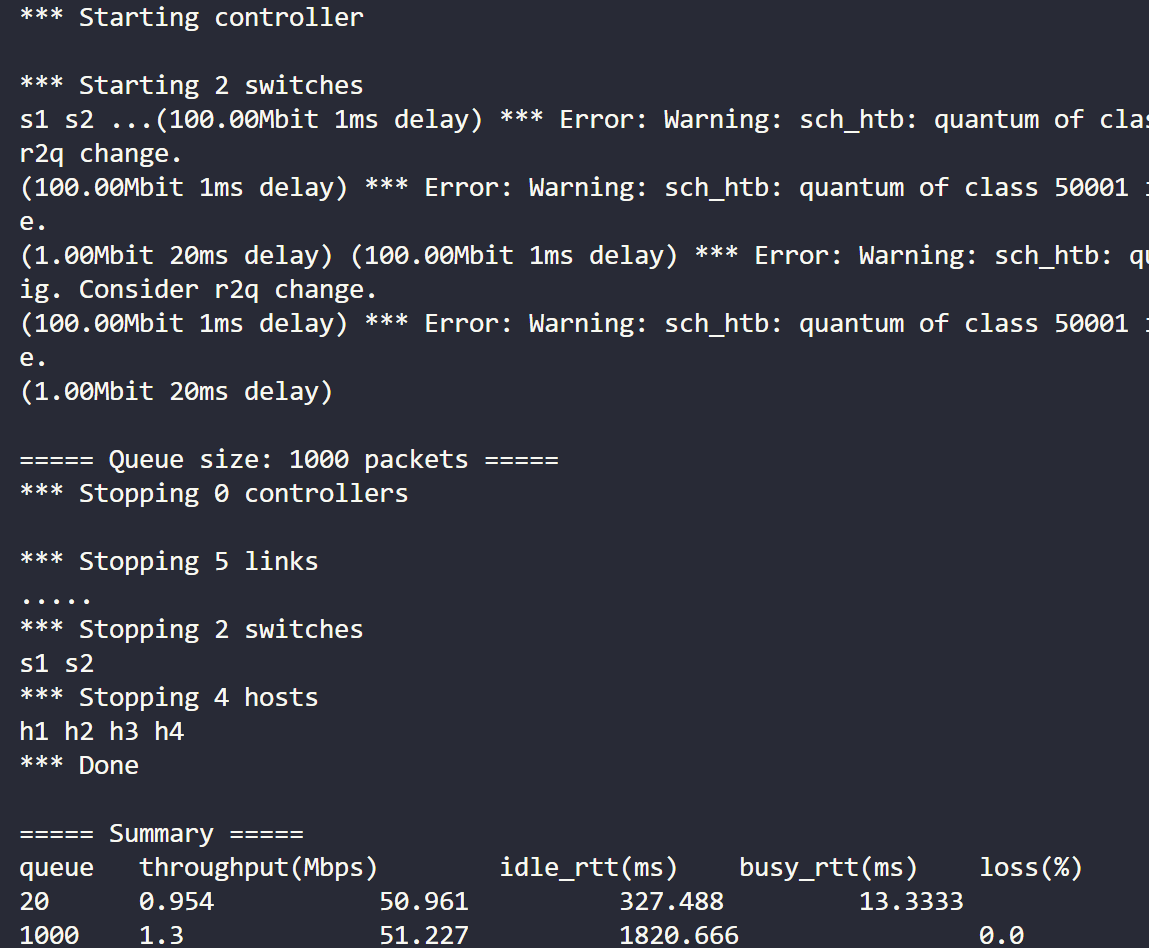
\includegraphics[width=0.82\textwidth]{img/bufferbloat.png}
    \caption{不同瓶颈队列大小下的 bufferbloat 实验结果。}
\end{figure}

\section{总结}

本项目实现了一个可运行的 SDN 控制器，将 DHCP、最短路径交换和防火墙功能集成在同一个 os-ken 应用中。整个实现由基于 Mininet 的测试支撑，并通过复杂拓扑与 bonus 实验进一步展示了系统在功能扩展和网络实验方面的能力。

最终报告应结合仓库中的测试脚本与演示文档一同阅读，尤其是复杂拓扑说明和现场答辩指南。

\end{document}
